% ============================================================
% M2 轮4 S3 · 练习件 第3课时（§1.1.2 空间向量基本定理）
% 题面：照题面库 成卷/题面库/课时03-1.1.2.md 全 16 题冻结入卷（卷面题号＝库序 1~16）；
%       组名/难度照库头第 3/4 字段（槽序冻结：难度与档位不单调，照登登记，不改槽）。
%       第13题库头标「多选」系源卷栏目习惯，题面为四选一（仅 B 真）→ 不标 \duoxuan，值钉 B。
%       第14题正方体记法顶底倒置已按定稿B §8.2 规范化为 ABCD-A₁B₁C₁D₁（改字不改果，落台账）。
% 模板基线＝练习线样张（六宏零改动拷入）；版式＝练习线 p2 课时训练
%       （\keshi＋multicols＋花形三档 基础巩固1~10／综合提升11~14／思维探索15~16）。
% 图源：第5题＝单元2 image3.png→dy2_image3.png(25mm)；第9题＝教材 p24(printed 17) 矢量图裁剪
%       →jc_lianxiB2.png(28mm)；第10题＝讲上 image6.png→js_image6.png(44mm)；
%       第13题＝讲上 image8.png→js_image8.png(40mm)；第14题＝单元2 image7.png→dy2_image7.png(30mm)。
% 取值/组名照登对照/图位/登记事项：见 ../批1值台账.md 课时03 节。
% 编译：xelatex main.tex（两遍）→ python render.py → png/pageN.png
% ============================================================
\documentclass[fontset=none]{ctexart}
\usepackage{qp-m3} % 换装：六宏→qp-m3 单包（钉后版 md5 7c3930362be8a0a2bdf21bbf8ac16573，两补钉随版）

% ============================================================
% 练习件局部宏（照练习线样张页2形制搬入；本段只加件，不改件）
% ============================================================
\renewcommand{\qpjianming}{练习件}
\renewcommand{\qpceming}{高中数学\quad 选择性必修第一册(人教B版)} % 换装回钉：qp-m3 默认册名＝选必二，防页脚漂移（试迁规约·试迁报告§四 B3 实证必改）
\renewcommand{\qpzhangming}{第一章\quad 空间向量与立体几何}

% ---------- YJ-01 灰块页脚·练习册档（块 31.0×7.8mm，照练习线样张 31.0mm 修正版） ----------
\newcommand{\qpxsyema}{\ifnum\value{page}<10 00\fi\ifnum\value{page}>9 \ifnum\value{page}<100 0\fi\fi\arabic{page}}
\newcommand{\lxshuziL}{\hbox to 13.8mm{\setlength{\fboxsep}{0pt}\colorbox{pnumbg}{%
  \makebox[31.0mm][l]{\rule[-3.145mm]{0pt}{7.8mm}\hspace{2.8mm}\fontsize{10.7pt}{13pt}\selectfont\color{black}\numpnum\qpxsyema}}\hss}}
\newcommand{\lxshuziR}{\hbox to 13.8mm{\kern-17.2mm\setlength{\fboxsep}{0pt}\colorbox{pnumbg}{%
  \makebox[31.0mm][r]{\rule[-3.145mm]{0pt}{7.8mm}\fontsize{10.7pt}{13pt}\selectfont\color{black}\numpnum\qpxsyema\hspace{2.75mm}}}}}
\fancyfoot[RO]{\raisebox{-1.24mm}[0pt][0pt]{\qphuitext\qpzhangming\quad{\heiti\qpjianming}\hspace{3mm}\lxshuziL}}
\fancyfoot[LE]{\raisebox{-1.24mm}[0pt][0pt]{\lxshuziR\hspace{3mm}\qphuitext\qpceming}}

% ---------- HX-01 花形·三档名（练习册版 25.5×6.8mm，重叠 o＝5.1mm） ----------
% 局部宏 \huadianOverlapLx 已由 qp-m3 收编（等值定义），依换装方案§1.4 预删防撞名
% 局部宏 \dangbadge 已由 qp-m3 收编（等值定义），依换装方案§1.4 预删防撞名

% ---------- TJ-02 练习册悬挂题号（单号 5.75mm／双位 7.6mm） ----------
% 长度 \lxhang 已由 qp-m3 分配，预删防重复定义
% 局部宏 \tihao 已由 qp-m3 收编（等值定义），依换装方案§1.4 预删防撞名
% 局部宏 \lxopt 已由 qp-m3 收编（等值定义），依换装方案§1.4 预删防撞名
% 局部宏 \xiexwei 已由 qp-m3 收编（等值定义），依换装方案§1.4 预删防撞名
% 局部宏 \zu 已由 qp-m3 收编（等值定义），依换装方案§1.4 预删防撞名

\begin{document}

% ============================================================
% 课时训练（三档 10＋4＋2＝16 题）
% ============================================================
\keshi{第3课时\quad 空间向量基本定理}
\begin{multicols}{2}
\emergencystretch=1em

\dangbadge{基}{础}{巩}{固}

\tihao{1}\zu{BC1 基底概念辨析×单选} \tieside{简单}若\(\{\overrightarrow{a},\overrightarrow{b},\overrightarrow{c}\}\)是空间的一个基底，则下列各组中不能构成空间的一个基底的是\nobreak(\kongwei)
\lxopt{A．\(\overrightarrow{a},2\overrightarrow{b},3\overrightarrow{c}\)；}
\lxopt{B．\(\overrightarrow{a}+\overrightarrow{b},\overrightarrow{b}+\overrightarrow{c},\overrightarrow{c}+\overrightarrow{a}\)；}
\lxopt{C．\(\overrightarrow{a}+\overrightarrow{b}+\overrightarrow{c},\overrightarrow{b}+\overrightarrow{c},\overrightarrow{c}\)；}
\lxopt{D．\(\overrightarrow{a}+2\overrightarrow{b},2\overrightarrow{b}+3\overrightarrow{c},3\overrightarrow{a}-9\overrightarrow{c}\)}
\begin{ansblock}[练-课时03-1]
% ans:练-课时03-1
\ansitem{1}{D}
\end{ansblock}

\tihao{2}\zu{BC1 命题组辨真假·计数选型} \tieside{简单}在以下三个命题中，真命题的个数是\nobreak(\kongwei)
\lxopt{①若三个非零向量\(\overrightarrow{a}\)，\(\overrightarrow{b}\)，\(\overrightarrow{c}\)不能构成空间的一个基底，则\(\overrightarrow{a}\)，\(\overrightarrow{b}\)，\(\overrightarrow{c}\)共面；}
\lxopt{②若两个非零向量\(\overrightarrow{a}\)，\(\overrightarrow{b}\)与任何一个向量都不能构成空间的一个基底，则\(\overrightarrow{a}\)，\(\overrightarrow{b}\)共线；}
\lxopt{③若\(\overrightarrow{a}\)，\(\overrightarrow{b}\)是两个不共线的向量，而\(\overrightarrow{c}=\lambda\overrightarrow{a}+\mu\overrightarrow{b}\)（\(\lambda\)，\(\mu\in\mathbf{R}\)且\(\lambda\mu\neq0\)），则\(\{\overrightarrow{a},\overrightarrow{b},\overrightarrow{c}\}\)构成空间的一个基底．}
\lxopt{\makebox[\dimexpr0.25\linewidth-0.5em\relax][l]{A．0；}\makebox[\dimexpr0.25\linewidth-0.5em\relax][l]{B．1；}\makebox[\dimexpr0.25\linewidth-0.5em\relax][l]{C．2；}\makebox[\dimexpr0.25\linewidth-0.5em\relax][l]{D．3}}
\begin{ansblock}[练-课时03-2]
% ans:练-课时03-2
\ansitem{2}{C（2 个真）}
\end{ansblock}

\tihao{3}\duoxuan\zu{BC2 基底存在性＋多点共面推理×多选} \tieside{简单}已知\(A\)，\(B\)，\(C\)，\(D\)，\(E\)是空间五点，且任何三点不共线．若\(\overrightarrow{AB}\)，\(\overrightarrow{AC}\)，\(\overrightarrow{AD}\)与\(\overrightarrow{AB}\)，\(\overrightarrow{AC}\)，\(\overrightarrow{AE}\)均不能构成空间的一个基底，则下列结论中正确的有(\kongwei)
\lxopt{A．\(\overrightarrow{AB}\)，\(\overrightarrow{AD}\)，\(\overrightarrow{AE}\)不能构成空间的一个基底；}
\lxopt{B．\(\overrightarrow{AC}\)，\(\overrightarrow{AD}\)，\(\overrightarrow{AE}\)不能构成空间的一个基底；}
\lxopt{C．\(\overrightarrow{BC}\)，\(\overrightarrow{CD}\)，\(\overrightarrow{DE}\)不能构成空间的一个基底；}
\lxopt{D．\(\overrightarrow{AB}\)，\(\overrightarrow{CD}\)，\(\overrightarrow{EA}\)能构成空间的一个基底}
\begin{ansblock}[练-课时03-3]
% ans:练-课时03-3
\ansitem{3}{ABC}
\end{ansblock}

\tihao{4}\duoxuan\zu{BC3 系数和＝1 判四点共面×多选} \tieside{简单}对空间任意一点\(O\)和不共线三点\(A\)，\(B\)，\(C\)，能得到\(P\)，\(A\)，\(B\)，\(C\)四点共面的是\nobreak(\kongwei)
\lxopt{A．\(\overrightarrow{OP}=\overrightarrow{OA}+\overrightarrow{OB}+\overrightarrow{OC}\)；}
\lxopt{B．\(\overrightarrow{OP}=\frac{1}{3}\overrightarrow{OA}+\frac{1}{3}\overrightarrow{OB}+\frac{1}{3}\overrightarrow{OC}\)；}
\lxopt{C．\(\overrightarrow{OP}=\frac{3}{4}\overrightarrow{OA}+\frac{1}{8}\overrightarrow{OB}+\frac{1}{8}\overrightarrow{OC}\)；}
\lxopt{D．\(\overrightarrow{OP}=2\overrightarrow{OA}-\overrightarrow{OB}-\overrightarrow{OC}\)}
\begin{ansblock}[练-课时03-4]
% ans:练-课时03-4
\ansitem{4}{BC}
\end{ansblock}

\tihao{5}\zu{BC5 用基底表示向量（双重中点）×单选} \tieside{简单}三棱柱\(ABC\text{-}\penalty100 DEF\)中，\(G\)为棱\(AD\)的中点，若\(\overrightarrow{BA}=\overrightarrow{a}\)，\(\overrightarrow{BC}=\overrightarrow{b}\)，\(\overrightarrow{BD}=\overrightarrow{c}\)，则\nobreak\(\overrightarrow{CG}=\)(\kongwei)
\par\vspace{1.9mm}\penalty10000\noindent\makebox[\linewidth][c]{
\includegraphics[width=25mm]{figs/dy2_image3.png}}\par\vspace{-1.0mm}\penalty10000
\lxopt{A．\(-\overrightarrow{a}+\overrightarrow{b}-\overrightarrow{c}\)；}
\lxopt{B．\(\frac{1}{2}\overrightarrow{a}-\overrightarrow{b}+\frac{1}{2}\overrightarrow{c}\)；}
\lxopt{C．\(-\frac{1}{2}\overrightarrow{a}+\overrightarrow{b}+\overrightarrow{c}\)；}
\lxopt{D．\(-\frac{1}{2}\overrightarrow{a}+\frac{1}{2}\overrightarrow{b}+\overrightarrow{c}\)}
\begin{ansblock}[练-课时03-5]
% ans:练-课时03-5
\ansitem{5}{B（\(\dfrac{1}{2}\overrightarrow{a}-\overrightarrow{b}+\dfrac{1}{2}\overrightarrow{c}\)）}
\end{ansblock}

\tihao{6}\zu{BC6 基底变换（坐标式系数对应）×单选} \tieside{简单}已知\(\{\overrightarrow{a},\overrightarrow{b},\overrightarrow{c}\}\)是空间向量的一个基底，\(\{\overrightarrow{a}+\overrightarrow{b},\overrightarrow{a}-\overrightarrow{b},\overrightarrow{c}\}\)是空间向量的另一个基底，若向量\(\overrightarrow{p}\)在基底\(\{\overrightarrow{a},\overrightarrow{b},\overrightarrow{c}\}\)下的坐标为\((4,2,3)\)，则向量\(\overrightarrow{p}\)在基底\(\{\overrightarrow{a}+\overrightarrow{b},\overrightarrow{a}-\overrightarrow{b},\overrightarrow{c}\}\)下的坐标为\nobreak(\kongwei)
\lxopt{\makebox[\dimexpr0.25\linewidth-0.5em\relax][l]{A．\((4,0,3)\)；}\makebox[\dimexpr0.25\linewidth-0.5em\relax][l]{B．\((1,2,3)\)；}\makebox[\dimexpr0.25\linewidth-0.5em\relax][l]{C．\((3,1,3)\)；}\makebox[\dimexpr0.25\linewidth-0.5em\relax][l]{D．\((2,1,3)\)}}
\begin{ansblock}[练-课时03-6]
% ans:练-课时03-6
\ansitem{6}{C（\((3,1,3)\)）}
\end{ansblock}

\tihao{7}\zu{BC6b 系数唯一分解（二维两未知）×填空} \tieside{简单}如果空间向量\(\overrightarrow{a}\)，\(\overrightarrow{b}\)不共线，且\(\overrightarrow{a}-y\overrightarrow{b}=x\overrightarrow{a}+3\overrightarrow{b}\)，求\(x\)，\(y\)的值．
\xiexwei{16mm}
\begin{ansblock}[练-课时03-7]
% ans:练-课时03-7
\ansitem{7}{\(x=1\)，\(y=-3\)}
\end{ansblock}

\tihao{8}\zu{BC6b 三维不共面三未知} \tieside{简单}如果空间向量\(\overrightarrow{a}\)，\(\overrightarrow{b}\)，\(\overrightarrow{c}\)不共面，且\(3\overrightarrow{a}-2\overrightarrow{b}+\overrightarrow{c}=x\overrightarrow{a}+y\overrightarrow{b}+z\overrightarrow{c}\)，求\(x\)，\(y\)，\(z\)的值．
\xiexwei{16mm}
\begin{ansblock}[练-课时03-8]
% ans:练-课时03-8
\ansitem{8}{\(x=3\)，\(y=-2\)，\(z=1\)}
\end{ansblock}

\tihao{9}\zu{BC5b 四面体双重中点基底表示×解答} \tieside{简单}如图，四面体\(O\text{-}\penalty100 ABC\)中，\(\overrightarrow{OA}=\overrightarrow{a}\)，\(\overrightarrow{OB}=\overrightarrow{b}\)，\(\overrightarrow{OC}=\overrightarrow{c}\)，\(D\)为\(BC\)的中点，\(E\)为\(AD\)的中点，将\(\overrightarrow{OE}\)用向量\(\overrightarrow{a}\)，\(\overrightarrow{b}\)，\(\overrightarrow{c}\)表示出来．
\par\vspace{1.9mm}\penalty10000\noindent\makebox[\linewidth][c]{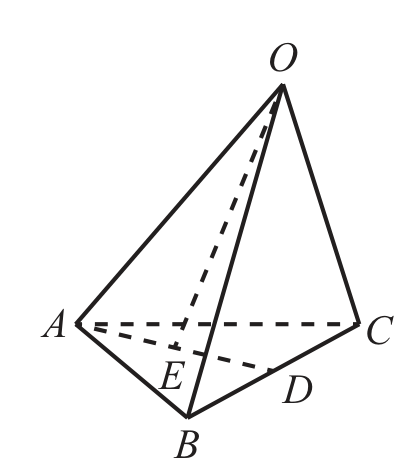
\includegraphics[width=28mm]{figs/jc_lianxiB2.png}}\par\vspace{-1.0mm}\penalty10000
\xiexwei{16mm}
\begin{ansblock}[练-课时03-9]
% ans:练-课时03-9
\ansitem{9}{\(\overrightarrow{OE}=\dfrac{1}{2}\overrightarrow{a}+\dfrac{1}{4}\overrightarrow{b}+\dfrac{1}{4}\overrightarrow{c}\)}
\end{ansblock}

\dangbadge{综}{合}{提}{升}

\tihao{10}\zu{BC4 四点共面证明＋基底分解求系数×解答} \tieside{中档}如图所示，在平行六面体\(ABCD\text{-}\penalty100 A_1B_1C_1D_1\)中，\(E\)，\(F\)分别在\(BB_1\)和\(DD_1\)上，且\(BE=\frac{1}{3}BB_1\)，\(DF=\frac{2}{3}DD_1\)．
\par\vspace{1.9mm}\penalty10000\noindent\makebox[\linewidth][c]{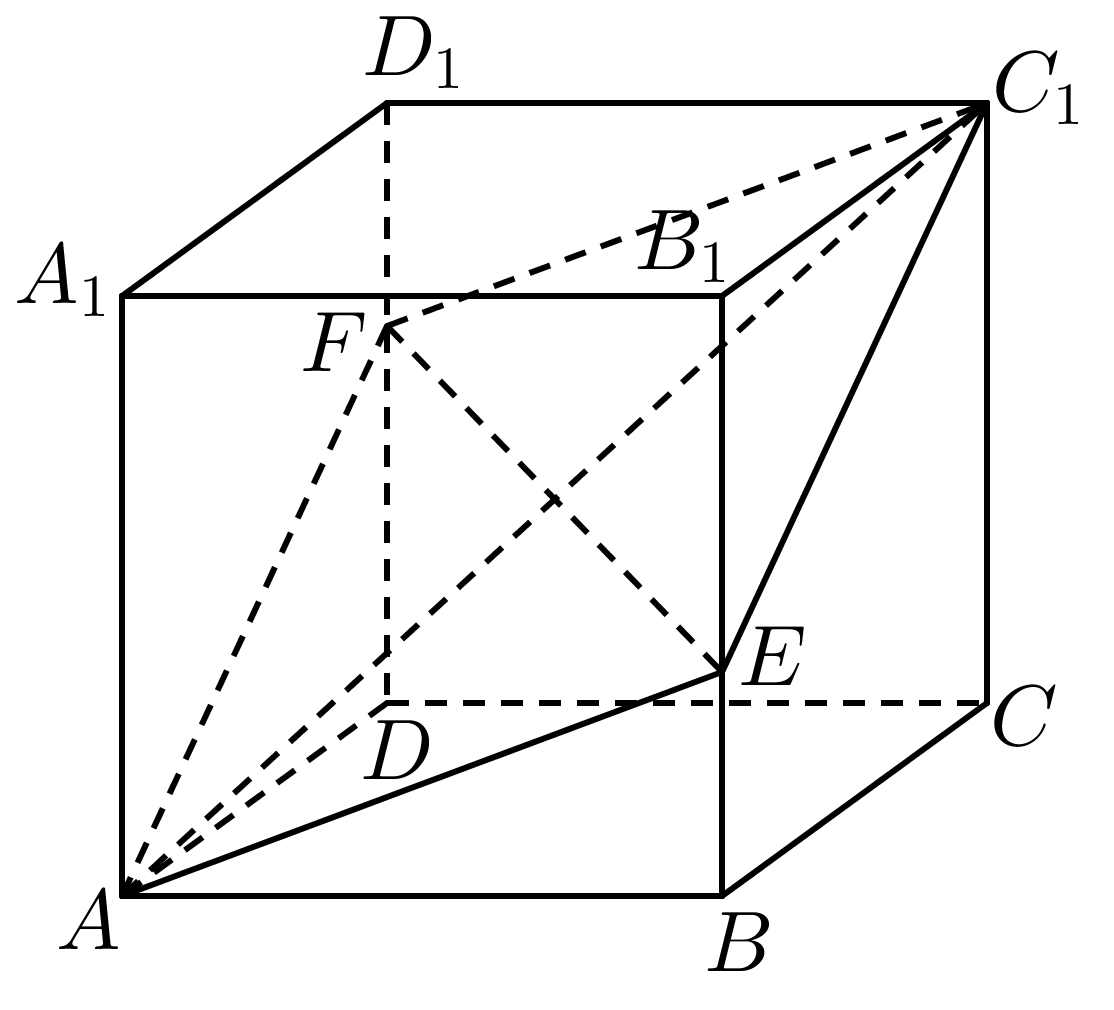
\includegraphics[width=44mm]{figs/js_image6.png}}\par\vspace{-1.0mm}\penalty10000
\lxopt{(1)证明：\(A\)，\(E\)，\(C_1\)，\(F\)四点共面．}
\lxopt{(2)若\(\overrightarrow{EF}=x\overrightarrow{AB}+y\overrightarrow{AD}+z\overrightarrow{AA_1}\)，求\(x+y+z\)．}
\xiexwei{16mm}
\begin{ansblock}[练-课时03-10]
% ans:练-课时03-10
\setlength{\anshang}{7.6mm}% 题10 起双位档（照答案册同值，块内局部）
\ansitem{10}{(1)证明 \(A\)、\(E\)、\(C_{1}\)、\(F\) 共面；(2)\(x+y+z=\dfrac{1}{3}\)}
\end{ansblock}

\tihao{11}\zu{BC7 共面向量定理反求参数×填空} \tieside{中档}已知\(\overrightarrow{i}\)，\(\overrightarrow{j}\)，\(\overrightarrow{k}\)是不共面向量，\(\overrightarrow{a}=2\overrightarrow{i}-\overrightarrow{j}+3\overrightarrow{k}\)，\(\overrightarrow{b}=-\overrightarrow{i}+4\overrightarrow{j}-2\overrightarrow{k}\)，\(\overrightarrow{c}=7\overrightarrow{i}+5\overrightarrow{j}+\lambda\overrightarrow{k}\)，若\(\overrightarrow{a}\)，\(\overrightarrow{b}\)，\(\overrightarrow{c}\)三个向量共面，则实数\(\lambda\)等于\kongbai{}．
\begin{ansblock}[练-课时03-11]
% ans:练-课时03-11
\setlength{\anshang}{7.6mm}% 题11 起双位档（照答案册同值，块内局部）
\ansitem{11}{\(\lambda=\dfrac{65}{7}\)}
\end{ansblock}

\tihao{12}\zu{BC5 重心条件三连分解×解答} \tieside{中档}已知\(PA\perp\)平面\(ABCD\)，四边形\(ABCD\)为正方形，\(G\)为\(\triangle PDC\)的重心，\(\overrightarrow{AB}=\overrightarrow{i}\)，\(\overrightarrow{AD}=\overrightarrow{j}\)，\(\overrightarrow{AP}=\overrightarrow{k}\)，试用基底\(\{\overrightarrow{i},\overrightarrow{j},\overrightarrow{k}\}\)表示\(\overrightarrow{PG}\)，\(\overrightarrow{BG}\)，\(\overrightarrow{AG}\)．
\xiexwei{16mm}
\begin{ansblock}[练-课时03-12]
% ans:练-课时03-12
\setlength{\anshang}{7.6mm}% 题12 起双位档（照答案册同值，块内局部）
\ansitem{12}{\(\overrightarrow{PG}=\dfrac{1}{3}\overrightarrow{i}+\dfrac{2}{3}\overrightarrow{j}-\dfrac{2}{3}\overrightarrow{k}\)；\(\overrightarrow{BG}=-\dfrac{2}{3}\overrightarrow{i}+\dfrac{2}{3}\overrightarrow{j}+\dfrac{1}{3}\overrightarrow{k}\)；\(\overrightarrow{AG}=\dfrac{1}{3}\overrightarrow{i}+\dfrac{2}{3}\overrightarrow{j}+\dfrac{1}{3}\overrightarrow{k}\)}
\end{ansblock}

\tihao{13}\zu{BC8 基底法数量积综合×多选} \tieside{中档}如图，一个结晶体的形状为平行六面体\(ABCD\text{-}\penalty100 A_1B_1C_1D_1\)，其中，以顶点\(A\)为端点的三条棱长均为\(6\)，且它们彼此的夹角都是\(60^\circ\)，下列说法中正确的是\nobreak(\kongwei)
\par\vspace{1.9mm}\penalty10000\noindent\makebox[\linewidth][c]{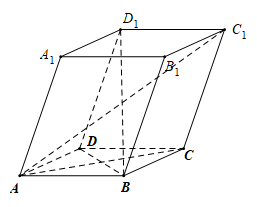
\includegraphics[width=40mm]{figs/js_image8.png}}\par\vspace{-1.0mm}\penalty10000
\lxopt{A．\(AC_1=6\)；}
\lxopt{B．\(AC_1\perp BD\)；}
\lxopt{C．向量\(\overrightarrow{B_1C}\)与\(\overrightarrow{AA_1}\)的夹角是\(60^\circ\)；}
\lxopt{D．\(BD_1\)与\(AC\)所成角的余弦值为\(\frac{\sqrt{6}}{3}\)}
\begin{ansblock}[练-课时03-13]
% ans:练-课时03-13
\setlength{\anshang}{7.6mm}% 题13 起双位档（照答案册同值，块内局部）
\ansitem{13}{B（\(AC_{1}\cdot BD=0\) 恒）}
\end{ansblock}

\tihao{14}\zu{四点共面证明×正方体双中点（1.2.2 拓展认领入简槽）} \tieside{简单}如图所示，在正方体\(ABCD\text{-}\penalty100 A_1B_1C_1D_1\)中，\(E\)，\(F\)分别是\(B_1C_1\)，\(C_1D_1\)的中点，求证：\(E\)，\(F\)，\(B\)，\(D\)四点共面．
\par\vspace{1.9mm}\penalty10000\noindent\makebox[\linewidth][c]{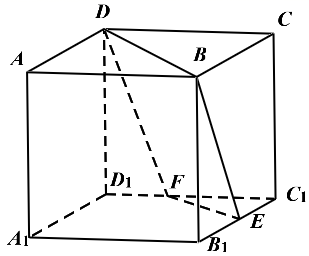
\includegraphics[width=30mm]{figs/dy2_image7.png}}\par\vspace{-1.0mm}\penalty10000
\xiexwei{16mm}
\begin{ansblock}[练-课时03-14]
% ans:练-课时03-14
\setlength{\anshang}{7.6mm}% 题14 起双位档（照答案册同值，块内局部）
\ansitem{14}{证明见解析}
\ansnote{解析}{\(EF\parallel B_{1}D_{1}\parallel BD\)，故共面。}
\end{ansblock}

\dangbadge{思}{维}{探}{索}

\tihao{15}\zu{BC-C2 组合判 p,q,r 共面·说理解答} \tieside{难}已知空间向量\(\overrightarrow{a}\)，\(\overrightarrow{b}\)，\(\overrightarrow{c}\)不共面，且\(\overrightarrow{p}=\overrightarrow{a}+\overrightarrow{b}\)，\(\overrightarrow{q}=\overrightarrow{a}+\overrightarrow{c}\)，\(\overrightarrow{r}=\overrightarrow{b}-\overrightarrow{c}\)，判断向量\(\overrightarrow{p}\)，\(\overrightarrow{q}\)，\(\overrightarrow{r}\)是否共面，并说明理由．
\xiexwei{16mm}
\begin{ansblock}[练-课时03-15]
% ans:练-课时03-15
\setlength{\anshang}{7.6mm}% 题15 起双位档（照答案册同值，块内局部）
\ansitem{15}{共面（\(\overrightarrow{p}-\overrightarrow{q}=\overrightarrow{b}-\overrightarrow{c}=\overrightarrow{r}\)）}
\end{ansblock}

\tihao{16}\zu{BC-C4 点在面内充要条件（x＋y＋z＝1）×证明} \tieside{难}已知\(A\)，\(B\)，\(C\)是空间中不共线的三点，\(O\)是空间中任意一点，求证：\(P\)在平面\(ABC\)内的充要条件是，存在满足\(x+y+z=1\)的实数\(x\)，\(y\)，\(z\)，使得\(\overrightarrow{OP}=x\overrightarrow{OA}+y\overrightarrow{OB}+z\overrightarrow{OC}\)．
\xiexwei{16mm}
\begin{ansblock}[练-课时03-16]
% ans:练-课时03-16
\setlength{\anshang}{7.6mm}% 题16 起双位档（照答案册同值，块内局部）
\ansitem{16}{充要条件证明}
\end{ansblock}

\end{multicols}

\tailfill
\end{document}
